\documentclass[twoside]{book}

% Packages required by doxygen
\usepackage{fixltx2e}
\usepackage{calc}
\usepackage{doxygen}
\usepackage[export]{adjustbox} % also loads graphicx
\usepackage{graphicx}
\usepackage[utf8]{inputenc}
\usepackage{makeidx}
\usepackage{multicol}
\usepackage{multirow}
\PassOptionsToPackage{warn}{textcomp}
\usepackage{textcomp}
\usepackage[nointegrals]{wasysym}
\usepackage[table]{xcolor}

% Font selection
\usepackage[T1]{fontenc}
\usepackage[scaled=.90]{helvet}
\usepackage{courier}
\usepackage{amssymb}
\usepackage{sectsty}
\renewcommand{\familydefault}{\sfdefault}
\allsectionsfont{%
  \fontseries{bc}\selectfont%
  \color{darkgray}%
}
\renewcommand{\DoxyLabelFont}{%
  \fontseries{bc}\selectfont%
  \color{darkgray}%
}
\newcommand{\+}{\discretionary{\mbox{\scriptsize$\hookleftarrow$}}{}{}}

% Page & text layout
\usepackage{geometry}
\geometry{%
  a4paper,%
  top=2.5cm,%
  bottom=2.5cm,%
  left=2.5cm,%
  right=2.5cm%
}
\tolerance=750
\hfuzz=15pt
\hbadness=750
\setlength{\emergencystretch}{15pt}
\setlength{\parindent}{0cm}
\setlength{\parskip}{3ex plus 2ex minus 2ex}
\makeatletter
\renewcommand{\paragraph}{%
  \@startsection{paragraph}{4}{0ex}{-1.0ex}{1.0ex}{%
    \normalfont\normalsize\bfseries\SS@parafont%
  }%
}
\renewcommand{\subparagraph}{%
  \@startsection{subparagraph}{5}{0ex}{-1.0ex}{1.0ex}{%
    \normalfont\normalsize\bfseries\SS@subparafont%
  }%
}
\makeatother

% Headers & footers
\usepackage{fancyhdr}
\pagestyle{fancyplain}
\fancyhead[LE]{\fancyplain{}{\bfseries\thepage}}
\fancyhead[CE]{\fancyplain{}{}}
\fancyhead[RE]{\fancyplain{}{\bfseries\leftmark}}
\fancyhead[LO]{\fancyplain{}{\bfseries\rightmark}}
\fancyhead[CO]{\fancyplain{}{}}
\fancyhead[RO]{\fancyplain{}{\bfseries\thepage}}
\fancyfoot[LE]{\fancyplain{}{}}
\fancyfoot[CE]{\fancyplain{}{}}
\fancyfoot[RE]{\fancyplain{}{\bfseries\scriptsize Generated by Doxygen }}
\fancyfoot[LO]{\fancyplain{}{\bfseries\scriptsize Generated by Doxygen }}
\fancyfoot[CO]{\fancyplain{}{}}
\fancyfoot[RO]{\fancyplain{}{}}
\renewcommand{\footrulewidth}{0.4pt}
\renewcommand{\chaptermark}[1]{%
  \markboth{#1}{}%
}
\renewcommand{\sectionmark}[1]{%
  \markright{\thesection\ #1}%
}

% Indices & bibliography
\usepackage{natbib}
\usepackage[titles]{tocloft}
\setcounter{tocdepth}{3}
\setcounter{secnumdepth}{5}
\makeindex

% Hyperlinks (required, but should be loaded last)
\usepackage{ifpdf}
\ifpdf
  \usepackage[pdftex,pagebackref=true]{hyperref}
\else
  \usepackage[ps2pdf,pagebackref=true]{hyperref}
\fi
\hypersetup{%
  colorlinks=true,%
  linkcolor=blue,%
  citecolor=blue,%
  unicode%
}

% Custom commands
\newcommand{\clearemptydoublepage}{%
  \newpage{\pagestyle{empty}\cleardoublepage}%
}

\usepackage{caption}
\captionsetup{labelsep=space,justification=centering,font={bf},singlelinecheck=off,skip=4pt,position=top}

%===== C O N T E N T S =====

\begin{document}

% Titlepage & ToC
\hypersetup{pageanchor=false,
             bookmarksnumbered=true,
             pdfencoding=unicode
            }
\pagenumbering{roman}
\begin{titlepage}
\vspace*{7cm}
\begin{center}%
{\Large Graph-\/\+L\+IB \\[1ex]\large 1 }\\
\vspace*{1cm}
{\large Generated by Doxygen 1.8.11}\\
\end{center}
\end{titlepage}
\clearemptydoublepage
\tableofcontents
\clearemptydoublepage
\pagenumbering{arabic}
\hypersetup{pageanchor=true}

%--- Begin generated contents ---
\chapter{Graphlib}
\label{index}\hypertarget{index}{}\hypertarget{index_Objective}{}\section{Objective}\label{index_Objective}
The purpose of this library is to provide a easy to use framework for various data structures and also to get some practise in writing code for different data structures and using different synchronization primitives \hypertarget{index_Status}{}\section{Status}\label{index_Status}
Currently there is a long way to go for the code, the basic framework is in place and athough the progress has been slow due to real life commitments, changes are being made intermittently. 
\chapter{Hierarchical Index}
\section{Class Hierarchy}
This inheritance list is sorted roughly, but not completely, alphabetically\-:\begin{DoxyCompactList}
\item \contentsline{section}{Graph$<$ Tnode, Tlink $>$}{\pageref{classGraph}}{}
\item \contentsline{section}{Link\-\_\-base}{\pageref{classLink__base}}{}
\begin{DoxyCompactList}
\item \contentsline{section}{Link$<$ Tlink, Tnode $>$}{\pageref{classLink}}{}
\item \contentsline{section}{Link$<$ Tnodelink, Tnode $>$}{\pageref{classLink}}{}
\end{DoxyCompactList}
\item \contentsline{section}{Node\-\_\-base}{\pageref{classNode__base}}{}
\begin{DoxyCompactList}
\item \contentsline{section}{Node$<$ Tnode, Tnodelink $>$}{\pageref{classNode}}{}
\item \contentsline{section}{Node$<$ Tnode, Tlink $>$}{\pageref{classNode}}{}
\end{DoxyCompactList}
\end{DoxyCompactList}

\chapter{Class Index}
\section{Class List}
Here are the classes, structs, unions and interfaces with brief descriptions\+:\begin{DoxyCompactList}
\item\contentsline{section}{\hyperlink{classGraph}{Graph$<$ Tnode, Tlink $>$} \\*\hyperlink{classGraph}{Graph} class }{\pageref{classGraph}}{}
\item\contentsline{section}{\hyperlink{classLink}{Link$<$ Tlink, Tnode $>$} \\*\hyperlink{classLink}{Link} Class }{\pageref{classLink}}{}
\item\contentsline{section}{\hyperlink{classLink__base}{Link\+\_\+base} }{\pageref{classLink__base}}{}
\item\contentsline{section}{\hyperlink{classNode}{Node$<$ Tnode, Tnodelink $>$} \\*\hyperlink{classNode}{Node} class }{\pageref{classNode}}{}
\item\contentsline{section}{\hyperlink{classNode__base}{Node\+\_\+base} }{\pageref{classNode__base}}{}
\item\contentsline{section}{\hyperlink{classTree}{Tree$<$ Tnode $>$} \\*\hyperlink{classTree}{Tree} class }{\pageref{classTree}}{}
\end{DoxyCompactList}

\chapter{File Index}
\section{File List}
Here is a list of all documented files with brief descriptions\+:\begin{DoxyCompactList}
\item\contentsline{section}{dev/inc/core/\hyperlink{common_8hpp}{common.\+hpp} }{\pageref{common_8hpp}}{}
\item\contentsline{section}{dev/inc/core/\hyperlink{graph_8hpp}{graph.\+hpp} }{\pageref{graph_8hpp}}{}
\item\contentsline{section}{dev/inc/core/\hyperlink{link_8hpp}{link.\+hpp} }{\pageref{link_8hpp}}{}
\item\contentsline{section}{dev/inc/core/\hyperlink{node_8hpp}{node.\+hpp} }{\pageref{node_8hpp}}{}
\item\contentsline{section}{dev/inc/diagnostic/quiet/{\bfseries err\+Handler.\+hpp} }{\pageref{quiet_2errHandler_8hpp}}{}
\item\contentsline{section}{dev/inc/diagnostic/verbose/{\bfseries err\+Handler.\+hpp} }{\pageref{verbose_2errHandler_8hpp}}{}
\item\contentsline{section}{dev/inc/ds/trees/\hyperlink{tree_8hpp}{tree.\+hpp} }{\pageref{tree_8hpp}}{}
\item\contentsline{section}{dev/src/\hyperlink{unitTest1_8cpp}{unit\+Test1.\+cpp} }{\pageref{unitTest1_8cpp}}{}
\end{DoxyCompactList}

\chapter{Class Documentation}
\hypertarget{classGraph}{\section{Graph Class Reference}
\label{classGraph}\index{Graph@{Graph}}
}
\subsection*{Public Member Functions}
\begin{DoxyCompactItemize}
\item 
\hypertarget{classGraph_ad16518c5057fefb3bca6cec54ddfc638}{{\bfseries Graph} (list$<$ \hyperlink{classNode}{Node} $\ast$ $>$, list$<$ \hyperlink{classLink}{Link} $\ast$ $>$)}\label{classGraph_ad16518c5057fefb3bca6cec54ddfc638}

\item 
\hypertarget{classGraph_a380c0e9b7bd2ad67e66d09ca2e9617c1}{int {\bfseries display\-Graph} ()}\label{classGraph_a380c0e9b7bd2ad67e66d09ca2e9617c1}

\item 
\hypertarget{classGraph_ab99fd82fc61e4ef1545bbe373b086ad0}{int {\bfseries create\-Link} ()}\label{classGraph_ab99fd82fc61e4ef1545bbe373b086ad0}

\item 
\hypertarget{classGraph_a4a5d7946ad3ae60e209528cff0c2b040}{int {\bfseries create\-Node} ()}\label{classGraph_a4a5d7946ad3ae60e209528cff0c2b040}

\item 
\hypertarget{classGraph_aeed286fdbecaeaa1dda9025020d277bb}{int {\bfseries destroy\-Link} (int lid)}\label{classGraph_aeed286fdbecaeaa1dda9025020d277bb}

\item 
\hypertarget{classGraph_a92ceb30bef1546092fd8ad644d19c708}{int {\bfseries destroy\-Node} (int nid)}\label{classGraph_a92ceb30bef1546092fd8ad644d19c708}

\item 
\hypertarget{classGraph_a19151ebc59fe3763e975a8b9efd11b97}{\hyperlink{classNode}{Node} $\ast$ {\bfseries get\-Node\-By\-Id} (int nid)}\label{classGraph_a19151ebc59fe3763e975a8b9efd11b97}

\item 
\hypertarget{classGraph_a67c51272c1b9abc3f7a7990a9b69fb21}{\hyperlink{classLink}{Link} $\ast$ {\bfseries get\-Link\-By\-Id} (int lid)}\label{classGraph_a67c51272c1b9abc3f7a7990a9b69fb21}

\item 
\hypertarget{classGraph_abb7ea2ae26c56a78993b16fc59eed565}{int {\bfseries attach\-Link\-To\-Node\-At\-Edge} (int lid, int nid, int edge)}\label{classGraph_abb7ea2ae26c56a78993b16fc59eed565}

\item 
\hypertarget{classGraph_a63da378eba2a985502ed63fb4c93b342}{int {\bfseries detach\-Link\-From\-Node\-At\-Edge} (int lid, int nid, int edge)}\label{classGraph_a63da378eba2a985502ed63fb4c93b342}

\end{DoxyCompactItemize}


The documentation for this class was generated from the following files\-:\begin{DoxyCompactItemize}
\item 
\hyperlink{graph_8hpp}{graph.\-hpp}\item 
\hyperlink{graph_8cpp}{graph.\-cpp}\end{DoxyCompactItemize}

\hypertarget{classLink}{\section{Link Class Reference}
\label{classLink}\index{Link@{Link}}
}


\hyperlink{classLink}{Link} Class.  




{\ttfamily \#include $<$link.\-hpp$>$}

\subsection*{Public Member Functions}
\begin{DoxyCompactItemize}
\item 
\hypertarget{classLink_a7d1f0fba2d522bae401cac8602820cce}{\hyperlink{classLink_a7d1f0fba2d522bae401cac8602820cce}{Link} (int weight=1)}\label{classLink_a7d1f0fba2d522bae401cac8602820cce}

\begin{DoxyCompactList}\small\item\em Constructor which initializes the weight to 1. \end{DoxyCompactList}\item 
\hypertarget{classLink_aac6fc336b263d742d2d72ccc28b8d34a}{int \hyperlink{classLink_aac6fc336b263d742d2d72ccc28b8d34a}{get\-Id} ()}\label{classLink_aac6fc336b263d742d2d72ccc28b8d34a}

\begin{DoxyCompactList}\small\item\em Member function which returns the unique index of the link. \end{DoxyCompactList}\item 
\hypertarget{classLink_aef6e5d265556b37090bb59e1bc842ede}{int \hyperlink{classLink_aef6e5d265556b37090bb59e1bc842ede}{add\-Node\-To\-Edge} (\hyperlink{classNode}{Node} $\ast$node, int edge)}\label{classLink_aef6e5d265556b37090bb59e1bc842ede}

\begin{DoxyCompactList}\small\item\em Member function used to add a \hyperlink{classNode}{Node} to one of the edges of the link. \end{DoxyCompactList}\item 
\hypertarget{classLink_ae70cfdb53e4e84f74fccf32672bba0ff}{int \hyperlink{classLink_ae70cfdb53e4e84f74fccf32672bba0ff}{node\-I\-D\-Attached\-To\-Edge} (int edge)}\label{classLink_ae70cfdb53e4e84f74fccf32672bba0ff}

\begin{DoxyCompactList}\small\item\em Member function that returns the node I\-D of the node attached to the specified edge. \end{DoxyCompactList}\item 
\hypertarget{classLink_a16589e17a3f22a5038b3c708d70bf5ea}{void \hyperlink{classLink_a16589e17a3f22a5038b3c708d70bf5ea}{detach\-Node\-By\-Edge} (int edge)}\label{classLink_a16589e17a3f22a5038b3c708d70bf5ea}

\begin{DoxyCompactList}\small\item\em Member function to detach the node attached to an edge of the link. \end{DoxyCompactList}\item 
\hypertarget{classLink_a901e3ffdb61055396977a5418d446535}{\hyperlink{classNode}{Node} $\ast$ \hyperlink{classLink_a901e3ffdb61055396977a5418d446535}{get\-Node\-At\-Edge} (int edge)}\label{classLink_a901e3ffdb61055396977a5418d446535}

\begin{DoxyCompactList}\small\item\em Member function that returns the \hyperlink{classNode}{Node} object at the given edge. \end{DoxyCompactList}\end{DoxyCompactItemize}
\subsection*{Friends}
\begin{DoxyCompactItemize}
\item 
\hypertarget{classLink_a1cccce22df97e21e1e0e0cd3ca6526b0}{int \hyperlink{classLink_a1cccce22df97e21e1e0e0cd3ca6526b0}{add\-Link\-Edge\-To\-Node} (\hyperlink{classNode}{Node} $\ast$node, \hyperlink{classLink}{Link} $\ast$link, int edge)}\label{classLink_a1cccce22df97e21e1e0e0cd3ca6526b0}

\begin{DoxyCompactList}\small\item\em Friend function to attach nodes to edges. \end{DoxyCompactList}\end{DoxyCompactItemize}


\subsection{Detailed Description}
\hyperlink{classLink}{Link} Class. 

The \hyperlink{classLink}{Link} class represents the link between two nodes. Each link has two edges, and the link itself has an integral weight. Two static integers are used to keep track of the number of links created and the link indices in use 

The documentation for this class was generated from the following files\-:\begin{DoxyCompactItemize}
\item 
link.\-hpp\item 
link.\-cpp\end{DoxyCompactItemize}

\hypertarget{classLink__base}{\section{Link\+\_\+base Class Reference}
\label{classLink__base}\index{Link\+\_\+base@{Link\+\_\+base}}
}
Inheritance diagram for Link\+\_\+base\+:\begin{figure}[H]
\begin{center}
\leavevmode
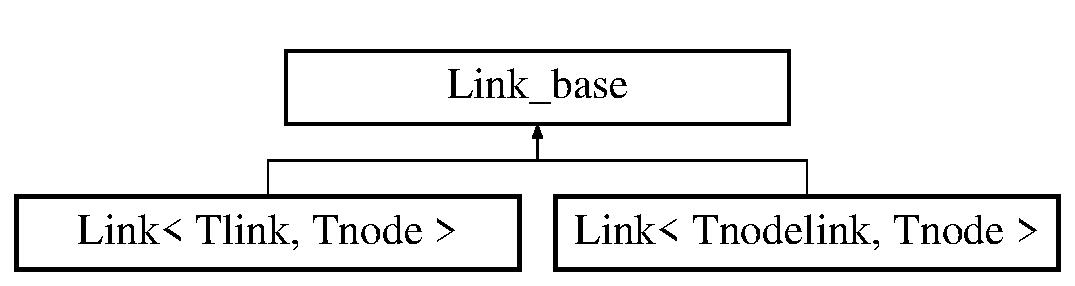
\includegraphics[height=2.000000cm]{classLink__base}
\end{center}
\end{figure}


The documentation for this class was generated from the following file\+:\begin{DoxyCompactItemize}
\item 
\hyperlink{common_8hpp}{common.\+hpp}\end{DoxyCompactItemize}

\hypertarget{classNode}{\section{Node$<$ Tnode, Tnodelink $>$ Class Template Reference}
\label{classNode}\index{Node$<$ Tnode, Tnodelink $>$@{Node$<$ Tnode, Tnodelink $>$}}
}


\hyperlink{classNode}{Node} class.  




{\ttfamily \#include $<$node.\-hpp$>$}

Inheritance diagram for Node$<$ Tnode, Tnodelink $>$\-:\begin{figure}[H]
\begin{center}
\leavevmode
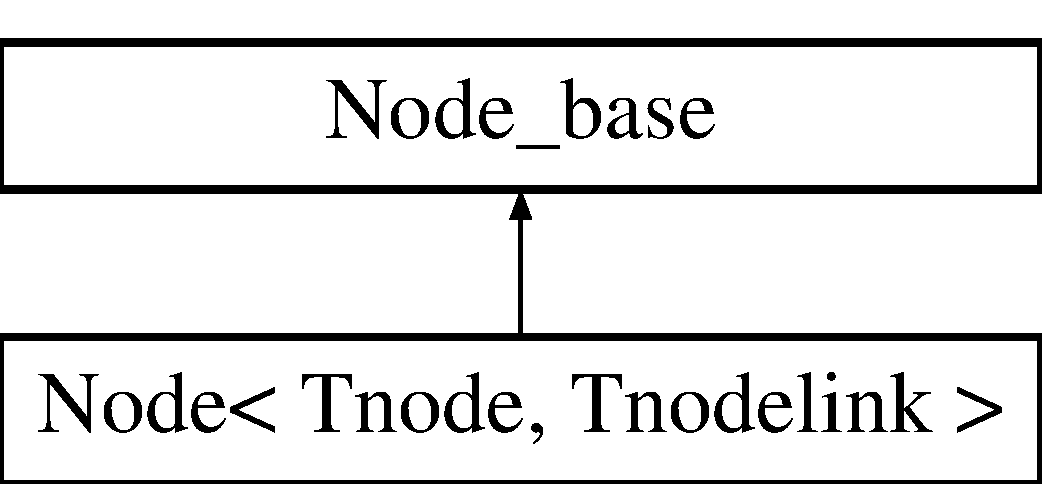
\includegraphics[height=2.000000cm]{classNode}
\end{center}
\end{figure}
\subsection*{Public Member Functions}
\begin{DoxyCompactItemize}
\item 
\hyperlink{classNode_a93fa08e2d8c63f93e3cc9ab8202e3334}{Node} ()
\begin{DoxyCompactList}\small\item\em \hyperlink{classNode}{Node} constructor which initializes the value to 0. \end{DoxyCompactList}\item 
\hyperlink{classNode_a5e6d51ef5b0456c3fd48b8196baebea5}{Node} (Tnode value)
\begin{DoxyCompactList}\small\item\em \hyperlink{classNode}{Node} constructor which initializes the value to 0. \end{DoxyCompactList}\item 
\hyperlink{classNode_a3bc7885a7623bde95ddd068d13c91af3}{$\sim$\-Node} ()
\begin{DoxyCompactList}\small\item\em Destructor which handles total\-\_\-nodes. \end{DoxyCompactList}\item 
int \hyperlink{classNode_a58fa0d9e8d2099bb0afd533d8ae55d12}{get\-Degree} ()
\begin{DoxyCompactList}\small\item\em Member function that returns the cardinality of the node. \end{DoxyCompactList}\item 
Tnode \hyperlink{classNode_aa9067e2137ecc75ddd802d5a574612f1}{get\-Value} ()
\begin{DoxyCompactList}\small\item\em Member function that returns the data in the node. \end{DoxyCompactList}\item 
int \hyperlink{classNode_a91639d810acda39b666715b07b5c2100}{get\-Id} ()
\begin{DoxyCompactList}\small\item\em Member function that returns the unique index of the node. \end{DoxyCompactList}\item 
void \hyperlink{classNode_a39ea9f0c2d3af467734b5c78a001bbcb}{set\-Value} (Tnode value)
\begin{DoxyCompactList}\small\item\em Member fuction that sets the value within the node. \end{DoxyCompactList}\item 
\hypertarget{classNode_a669f230accdef7328ef0c217c63b0dd4}{int \hyperlink{classNode_a669f230accdef7328ef0c217c63b0dd4}{add\-Link\-Edge} (\hyperlink{classLink}{Link}$<$ Tnodelink, Tnode $>$ $\ast$link, int edge)}\label{classNode_a669f230accdef7328ef0c217c63b0dd4}

\begin{DoxyCompactList}\small\item\em Member function that adds a particular edge of a link to the node. \end{DoxyCompactList}\item 
boolean \hyperlink{classNode_a9237bd16a22ee02c244d8cc95d6533bd}{link\-Attached\-To\-Node} (\hyperlink{classLink}{Link}$<$ Tnodelink, Tnode $>$ $\ast$link)
\begin{DoxyCompactList}\small\item\em Member function that returns whether or not a link is attached to the node. \end{DoxyCompactList}\item 
\hypertarget{classNode_ad469f4b48294f360d372b5765eee4f77}{int \hyperlink{classNode_ad469f4b48294f360d372b5765eee4f77}{remove\-Link\-Edge} (\hyperlink{classLink}{Link}$<$ Tnodelink, Tnode $>$ $\ast$link, int edge)}\label{classNode_ad469f4b48294f360d372b5765eee4f77}

\begin{DoxyCompactList}\small\item\em Member function to remove a link from the node at a particular edge. \end{DoxyCompactList}\item 
int \hyperlink{classNode_aa7a762ea839eea52e9d2cae7f31780e8}{remove\-Link} (\hyperlink{classLink}{Link}$<$ Tnodelink, Tnode $>$ $\ast$link)
\begin{DoxyCompactList}\small\item\em Member function to remove a link from the node at any edge. \end{DoxyCompactList}\end{DoxyCompactItemize}
\subsection*{Private Attributes}
\begin{DoxyCompactItemize}
\item 
\hypertarget{classNode_aff1733d2326817871268b920f5a981ca}{list$<$ \hyperlink{classLink}{Link}$<$ Tnodelink, Tnode $>$ $\ast$ $>$ \hyperlink{classNode_aff1733d2326817871268b920f5a981ca}{links\-\_\-}}\label{classNode_aff1733d2326817871268b920f5a981ca}

\begin{DoxyCompactList}\small\item\em The list of links that a particular node shares with the other nodes in the graph. \end{DoxyCompactList}\item 
\hypertarget{classNode_a78be1747ae96cf39fe2a9ae3be5212a4}{Tnode \hyperlink{classNode_a78be1747ae96cf39fe2a9ae3be5212a4}{value\-\_\-}}\label{classNode_a78be1747ae96cf39fe2a9ae3be5212a4}

\begin{DoxyCompactList}\small\item\em The data that a paprticular node holds. \end{DoxyCompactList}\item 
\hypertarget{classNode_a84fb338de56e4906d251f16bf27ee00f}{int \hyperlink{classNode_a84fb338de56e4906d251f16bf27ee00f}{node\-\_\-id\-\_\-}}\label{classNode_a84fb338de56e4906d251f16bf27ee00f}

\begin{DoxyCompactList}\small\item\em The unique index of a particular node. \end{DoxyCompactList}\item 
\hypertarget{classNode_af75893cb178fdcdd805df2d17c16a88b}{mutex \hyperlink{classNode_af75893cb178fdcdd805df2d17c16a88b}{links\-\_\-mutex\-\_\-}}\label{classNode_af75893cb178fdcdd805df2d17c16a88b}

\begin{DoxyCompactList}\small\item\em A mutex to protect access to the list of links from this node. \end{DoxyCompactList}\item 
\hypertarget{classNode_a846c5acc1ea3bfa722309b5b2ef8072e}{mutex \hyperlink{classNode_a846c5acc1ea3bfa722309b5b2ef8072e}{value\-\_\-mutex\-\_\-}}\label{classNode_a846c5acc1ea3bfa722309b5b2ef8072e}

\begin{DoxyCompactList}\small\item\em A mutex to protect the value in the node. \end{DoxyCompactList}\item 
\hypertarget{classNode_aa2e8d02482477aa2f05db0e6bb409339}{mutex \hyperlink{classNode_aa2e8d02482477aa2f05db0e6bb409339}{node\-\_\-id\-\_\-mutex\-\_\-}}\label{classNode_aa2e8d02482477aa2f05db0e6bb409339}

\begin{DoxyCompactList}\small\item\em A mutex to protect node\-\_\-id\-\_\-. \end{DoxyCompactList}\end{DoxyCompactItemize}
\subsection*{Static Private Attributes}
\begin{DoxyCompactItemize}
\item 
\hypertarget{classNode_a7f128d924b8d003fd03b258a99e71a67}{static int \hyperlink{classNode_a7f128d924b8d003fd03b258a99e71a67}{total\-\_\-nodes}}\label{classNode_a7f128d924b8d003fd03b258a99e71a67}

\begin{DoxyCompactList}\small\item\em A static member that keeps track of the total number of active nodes. \end{DoxyCompactList}\item 
\hypertarget{classNode_a280f4f7c00e3b9755bd0b47c3d0a91b7}{static int \hyperlink{classNode_a280f4f7c00e3b9755bd0b47c3d0a91b7}{total\-\_\-node\-\_\-ids}}\label{classNode_a280f4f7c00e3b9755bd0b47c3d0a91b7}

\begin{DoxyCompactList}\small\item\em A static member that tracks node indices in the graph. \end{DoxyCompactList}\item 
\hypertarget{classNode_a4ee6b9388653c1d3b1d94c7b91b40253}{static mutex \hyperlink{classNode_a4ee6b9388653c1d3b1d94c7b91b40253}{total\-\_\-nodes\-\_\-mutex}}\label{classNode_a4ee6b9388653c1d3b1d94c7b91b40253}

\begin{DoxyCompactList}\small\item\em A mutex to protect total\-\_\-nodes. \end{DoxyCompactList}\item 
\hypertarget{classNode_ac18d36beb867879f0a319557e783e146}{static mutex \hyperlink{classNode_ac18d36beb867879f0a319557e783e146}{total\-\_\-node\-\_\-ids\-\_\-mutex}}\label{classNode_ac18d36beb867879f0a319557e783e146}

\begin{DoxyCompactList}\small\item\em A mutex to protect total\-\_\-node\-\_\-ids. \end{DoxyCompactList}\end{DoxyCompactItemize}
\subsection*{Friends}
\begin{DoxyCompactItemize}
\item 
\hypertarget{classNode_a73e2a6b342470c352a5bd3843e75d475}{class \hyperlink{classNode_a73e2a6b342470c352a5bd3843e75d475}{Graph$<$ Tnode, Tnodelink $>$}}\label{classNode_a73e2a6b342470c352a5bd3843e75d475}

\begin{DoxyCompactList}\small\item\em Fried class \hyperlink{classGraph}{Graph}. \end{DoxyCompactList}\end{DoxyCompactItemize}


\subsection{Detailed Description}
\subsubsection*{template$<$class Tnode, class Tnodelink$>$class Node$<$ Tnode, Tnodelink $>$}

\hyperlink{classNode}{Node} class. 

This class represents each of the nodes of the graph. Each node has a list of links that it shares with other nodes A node is attached to another node by the link that it shares with the other node. Each node has an integer as its data 

\subsection{Constructor \& Destructor Documentation}
\hypertarget{classNode_a93fa08e2d8c63f93e3cc9ab8202e3334}{\index{Node@{Node}!Node@{Node}}
\index{Node@{Node}!Node@{Node}}
\subsubsection[{Node}]{\setlength{\rightskip}{0pt plus 5cm}template$<$class Tnode, class Tnodelink$>$ {\bf Node}$<$ Tnode, Tnodelink $>$\-::{\bf Node} (
\begin{DoxyParamCaption}
{}
\end{DoxyParamCaption}
)}}\label{classNode_a93fa08e2d8c63f93e3cc9ab8202e3334}


\hyperlink{classNode}{Node} constructor which initializes the value to 0. 

Default constructor \-: Just set the node\-\_\-id\-\_\- and update the tota nodes and total node ids. \hypertarget{classNode_a5e6d51ef5b0456c3fd48b8196baebea5}{\index{Node@{Node}!Node@{Node}}
\index{Node@{Node}!Node@{Node}}
\subsubsection[{Node}]{\setlength{\rightskip}{0pt plus 5cm}template$<$class Tnode, class Tnodelink$>$ {\bf Node}$<$ Tnode, Tnodelink $>$\-::{\bf Node} (
\begin{DoxyParamCaption}
\item[{Tnode}]{value}
\end{DoxyParamCaption}
)}}\label{classNode_a5e6d51ef5b0456c3fd48b8196baebea5}


\hyperlink{classNode}{Node} constructor which initializes the value to 0. 

Constructor to set the value and node\-\_\-id\-\_\-. Also update the total nodes and total node ids. \hypertarget{classNode_a3bc7885a7623bde95ddd068d13c91af3}{\index{Node@{Node}!$\sim$\-Node@{$\sim$\-Node}}
\index{$\sim$\-Node@{$\sim$\-Node}!Node@{Node}}
\subsubsection[{$\sim$\-Node}]{\setlength{\rightskip}{0pt plus 5cm}template$<$class Tnode, class Tnodelink$>$ {\bf Node}$<$ Tnode, Tnodelink $>$\-::$\sim${\bf Node} (
\begin{DoxyParamCaption}
{}
\end{DoxyParamCaption}
)}}\label{classNode_a3bc7885a7623bde95ddd068d13c91af3}


Destructor which handles total\-\_\-nodes. 

Destructor. 

\subsection{Member Function Documentation}
\hypertarget{classNode_a58fa0d9e8d2099bb0afd533d8ae55d12}{\index{Node@{Node}!get\-Degree@{get\-Degree}}
\index{get\-Degree@{get\-Degree}!Node@{Node}}
\subsubsection[{get\-Degree}]{\setlength{\rightskip}{0pt plus 5cm}template$<$class Tnode, class Tnodelink$>$ {\bf Node}$<$ Tnode, Tnodelink $>$\-::get\-Degree (
\begin{DoxyParamCaption}
{}
\end{DoxyParamCaption}
)}}\label{classNode_a58fa0d9e8d2099bb0afd533d8ae55d12}


Member function that returns the cardinality of the node. 

Returns the degree of a node by counting the number of links it is attached to. \hypertarget{classNode_a91639d810acda39b666715b07b5c2100}{\index{Node@{Node}!get\-Id@{get\-Id}}
\index{get\-Id@{get\-Id}!Node@{Node}}
\subsubsection[{get\-Id}]{\setlength{\rightskip}{0pt plus 5cm}template$<$class Tnode, class Tnodelink$>$ {\bf Node}$<$ Tnode, Tnodelink $>$\-::get\-Id (
\begin{DoxyParamCaption}
{}
\end{DoxyParamCaption}
)}}\label{classNode_a91639d810acda39b666715b07b5c2100}


Member function that returns the unique index of the node. 

Returns the node\-\_\-id\-\_\-. \hypertarget{classNode_aa9067e2137ecc75ddd802d5a574612f1}{\index{Node@{Node}!get\-Value@{get\-Value}}
\index{get\-Value@{get\-Value}!Node@{Node}}
\subsubsection[{get\-Value}]{\setlength{\rightskip}{0pt plus 5cm}template$<$class Tnode, class Tnodelink$>$ {\bf Node}$<$ Tnode, Tnodelink $>$\-::get\-Value (
\begin{DoxyParamCaption}
{}
\end{DoxyParamCaption}
)}}\label{classNode_aa9067e2137ecc75ddd802d5a574612f1}


Member function that returns the data in the node. 

Returns the value saved in the node. \hypertarget{classNode_a9237bd16a22ee02c244d8cc95d6533bd}{\index{Node@{Node}!link\-Attached\-To\-Node@{link\-Attached\-To\-Node}}
\index{link\-Attached\-To\-Node@{link\-Attached\-To\-Node}!Node@{Node}}
\subsubsection[{link\-Attached\-To\-Node}]{\setlength{\rightskip}{0pt plus 5cm}template$<$class Tnode, class Tnodelink$>$ {\bf Node}$<$ Tnode, Tnodelink $>$\-::link\-Attached\-To\-Node (
\begin{DoxyParamCaption}
\item[{{\bf Link}$<$ Tnodelink, Tnode $>$ $\ast$}]{link}
\end{DoxyParamCaption}
)}}\label{classNode_a9237bd16a22ee02c244d8cc95d6533bd}


Member function that returns whether or not a link is attached to the node. 

returns T\-R\-U\-E if passed link is attached to the node, else returns F\-A\-L\-S\-E. \hypertarget{classNode_aa7a762ea839eea52e9d2cae7f31780e8}{\index{Node@{Node}!remove\-Link@{remove\-Link}}
\index{remove\-Link@{remove\-Link}!Node@{Node}}
\subsubsection[{remove\-Link}]{\setlength{\rightskip}{0pt plus 5cm}template$<$class Tnode, class Tnodelink$>$ {\bf Node}$<$ Tnode, Tnodelink $>$\-::remove\-Link (
\begin{DoxyParamCaption}
\item[{{\bf Link}$<$ Tnodelink, Tnode $>$ $\ast$}]{link}
\end{DoxyParamCaption}
)}}\label{classNode_aa7a762ea839eea52e9d2cae7f31780e8}


Member function to remove a link from the node at any edge. 

Removes the passed link from the \hyperlink{classNode}{Node} and returns 0 on success, if link is not found, returns -\/1. \hypertarget{classNode_a39ea9f0c2d3af467734b5c78a001bbcb}{\index{Node@{Node}!set\-Value@{set\-Value}}
\index{set\-Value@{set\-Value}!Node@{Node}}
\subsubsection[{set\-Value}]{\setlength{\rightskip}{0pt plus 5cm}template$<$class Tnode, class Tnodelink$>$ {\bf Node}$<$ Tnode, Tnodelink $>$\-::set\-Value (
\begin{DoxyParamCaption}
\item[{Tnode}]{value}
\end{DoxyParamCaption}
)}}\label{classNode_a39ea9f0c2d3af467734b5c78a001bbcb}


Member fuction that sets the value within the node. 

Sets the value of the node. 

The documentation for this class was generated from the following file\-:\begin{DoxyCompactItemize}
\item 
\hyperlink{node_8hpp}{node.\-hpp}\end{DoxyCompactItemize}

\hypertarget{classNode__base}{\section{Node\+\_\+base Class Reference}
\label{classNode__base}\index{Node\+\_\+base@{Node\+\_\+base}}
}
Inheritance diagram for Node\+\_\+base\+:\begin{figure}[H]
\begin{center}
\leavevmode
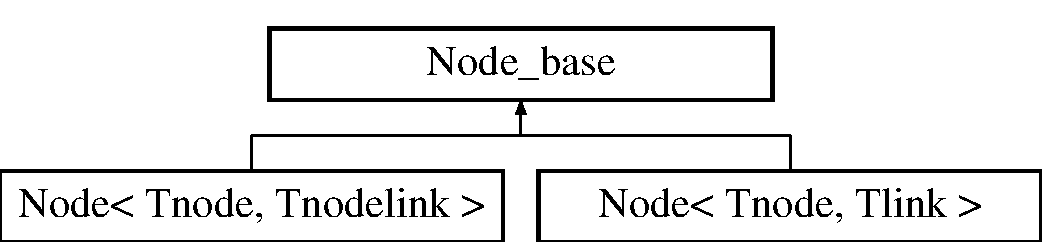
\includegraphics[height=2.000000cm]{classNode__base}
\end{center}
\end{figure}


The documentation for this class was generated from the following file\+:\begin{DoxyCompactItemize}
\item 
\hyperlink{common_8hpp}{common.\+hpp}\end{DoxyCompactItemize}

\hypertarget{classTree}{}\section{Tree$<$ Tnode $>$ Class Template Reference}
\label{classTree}\index{Tree$<$ Tnode $>$@{Tree$<$ Tnode $>$}}


\hyperlink{classTree}{Tree} class.  




{\ttfamily \#include $<$tree.\+hpp$>$}

Inheritance diagram for Tree$<$ Tnode $>$\+:\begin{figure}[H]
\begin{center}
\leavevmode
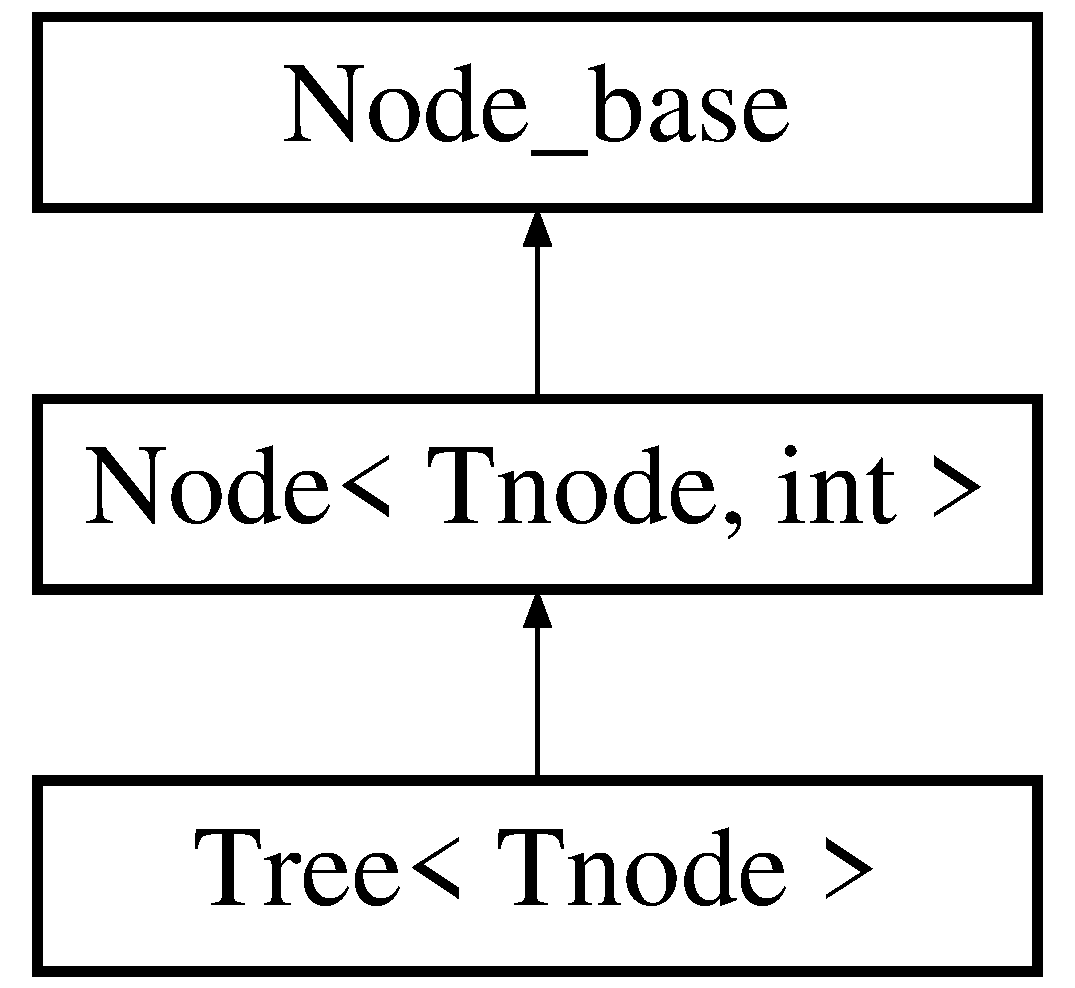
\includegraphics[height=3.000000cm]{classTree}
\end{center}
\end{figure}
\subsection*{Public Types}
\begin{DoxyCompactItemize}
\item 
enum {\bfseries Consts} \{ {\bfseries L\+E\+F\+T\+\_\+\+L\+I\+NK} = 0, 
{\bfseries R\+I\+G\+H\+T\+\_\+\+L\+I\+NK} = 1, 
{\bfseries P\+A\+R\+E\+N\+T\+\_\+\+L\+I\+NK} = 2, 
{\bfseries N\+U\+M\+\_\+\+L\+I\+N\+KS} = 3
 \}\hypertarget{classTree_a8d1e12815beb46a052311a85390f3d37}{}\label{classTree_a8d1e12815beb46a052311a85390f3d37}

\end{DoxyCompactItemize}
\subsection*{Public Member Functions}
\begin{DoxyCompactItemize}
\item 
\hyperlink{classTree_a66090705b8fb60acdbc3c7396a84931f}{Tree} ()\hypertarget{classTree_a66090705b8fb60acdbc3c7396a84931f}{}\label{classTree_a66090705b8fb60acdbc3c7396a84931f}

\begin{DoxyCompactList}\small\item\em Constructor. \end{DoxyCompactList}\item 
\hyperlink{classTree_a58625504ac52cc2ac7ba1f574ee1f856}{$\sim$\+Tree} ()\hypertarget{classTree_a58625504ac52cc2ac7ba1f574ee1f856}{}\label{classTree_a58625504ac52cc2ac7ba1f574ee1f856}

\begin{DoxyCompactList}\small\item\em Destructor. \end{DoxyCompactList}\item 
\hyperlink{classTree_aa1927536852f0e867af1c4259ea6e58b}{Tree} (Tnode val)\hypertarget{classTree_aa1927536852f0e867af1c4259ea6e58b}{}\label{classTree_aa1927536852f0e867af1c4259ea6e58b}

\begin{DoxyCompactList}\small\item\em Constructor. \end{DoxyCompactList}\item 
void \hyperlink{classTree_a6722213d27f3c4da7b127673283a6ea0}{traverse\+In\+Order} ()\hypertarget{classTree_a6722213d27f3c4da7b127673283a6ea0}{}\label{classTree_a6722213d27f3c4da7b127673283a6ea0}

\begin{DoxyCompactList}\small\item\em Traversal \+: Different orders of traversal. \end{DoxyCompactList}\item 
void {\bfseries traverse\+Pre\+Order} ()\hypertarget{classTree_a78c440a2fac8d4ad77bb4d13ba3a70e2}{}\label{classTree_a78c440a2fac8d4ad77bb4d13ba3a70e2}

\item 
void {\bfseries traverse\+Post\+Order} ()\hypertarget{classTree_a89dd922017d606826e516d0f52d824a8}{}\label{classTree_a89dd922017d606826e516d0f52d824a8}

\item 
int \hyperlink{classTree_a278f7564b09dc1600dcdb0cc4d3054a0}{create\+And\+Add\+Node\+On\+Left} (Tnode val)\hypertarget{classTree_a278f7564b09dc1600dcdb0cc4d3054a0}{}\label{classTree_a278f7564b09dc1600dcdb0cc4d3054a0}

\begin{DoxyCompactList}\small\item\em Create a node and add it to the tree on the left side. \end{DoxyCompactList}\item 
int \hyperlink{classTree_a44eb3341bc7ed66f255e9fe468ab06eb}{create\+And\+Add\+Node\+On\+Right} (Tnode val)\hypertarget{classTree_a44eb3341bc7ed66f255e9fe468ab06eb}{}\label{classTree_a44eb3341bc7ed66f255e9fe468ab06eb}

\begin{DoxyCompactList}\small\item\em Create a node and add it to the tree on the right side. \end{DoxyCompactList}\item 
\hyperlink{classTree}{Tree}$<$ Tnode $>$ $\ast$ \hyperlink{classTree_ae3f7bd77cb5a97850610d8467e92b4a6}{get\+Left\+Child} ()\hypertarget{classTree_ae3f7bd77cb5a97850610d8467e92b4a6}{}\label{classTree_ae3f7bd77cb5a97850610d8467e92b4a6}

\begin{DoxyCompactList}\small\item\em Get the Left child of the node. \end{DoxyCompactList}\item 
\hyperlink{classTree}{Tree}$<$ Tnode $>$ $\ast$ \hyperlink{classTree_acc04c93b0cead87c1cf2ddcaadcc3753}{get\+Right\+Child} ()\hypertarget{classTree_acc04c93b0cead87c1cf2ddcaadcc3753}{}\label{classTree_acc04c93b0cead87c1cf2ddcaadcc3753}

\begin{DoxyCompactList}\small\item\em Get the right child of the node. \end{DoxyCompactList}\item 
void \hyperlink{classTree_aa3d6fdeadd512395b1e2511dfc45936d}{delete\+Left\+Child} ()\hypertarget{classTree_aa3d6fdeadd512395b1e2511dfc45936d}{}\label{classTree_aa3d6fdeadd512395b1e2511dfc45936d}

\begin{DoxyCompactList}\small\item\em Delete the left child of the node, it will delete all the children of the children also. \end{DoxyCompactList}\item 
void \hyperlink{classTree_a6e3a484d9f7f10a3897502f77bd1532a}{delete\+Right\+Child} ()\hypertarget{classTree_a6e3a484d9f7f10a3897502f77bd1532a}{}\label{classTree_a6e3a484d9f7f10a3897502f77bd1532a}

\begin{DoxyCompactList}\small\item\em Delete the right child of the node, it will delete all the children of the children also. \end{DoxyCompactList}\end{DoxyCompactItemize}
\subsection*{Additional Inherited Members}


\subsection{Detailed Description}
\subsubsection*{template$<$class Tnode$>$\\*
class Tree$<$ Tnode $>$}

\hyperlink{classTree}{Tree} class. 

This class is for a binary tree data structure. It derives from the node class and maintains at most two children per node. It can be extended to also implement a parent pointer in the child nodes. 

The documentation for this class was generated from the following file\+:\begin{DoxyCompactItemize}
\item 
dev/inc/ds/trees/\hyperlink{tree_8hpp}{tree.\+hpp}\end{DoxyCompactItemize}

\chapter{File Documentation}
\hypertarget{common_8hpp}{}\section{dev/inc/core/common.hpp File Reference}
\label{common_8hpp}\index{dev/inc/core/common.\+hpp@{dev/inc/core/common.\+hpp}}
\subsection*{Classes}
\begin{DoxyCompactItemize}
\item 
class \hyperlink{classNode__base}{Node\+\_\+base}
\item 
class \hyperlink{classLink__base}{Link\+\_\+base}
\end{DoxyCompactItemize}
\subsection*{Enumerations}
\begin{DoxyCompactItemize}
\item 
enum {\bfseries boolean} \{ {\bfseries F\+A\+L\+SE}, 
{\bfseries T\+R\+UE}
 \}\hypertarget{common_8hpp_a7c6368b321bd9acd0149b030bb8275ed}{}\label{common_8hpp_a7c6368b321bd9acd0149b030bb8275ed}

\end{DoxyCompactItemize}

\hypertarget{graph_8hpp}{\section{graph.\-hpp File Reference}
\label{graph_8hpp}\index{graph.\-hpp@{graph.\-hpp}}
}
{\ttfamily \#include \char`\"{}common.\-hpp\char`\"{}}\\*
{\ttfamily \#include \char`\"{}node.\-hpp\char`\"{}}\\*
{\ttfamily \#include \char`\"{}link.\-hpp\char`\"{}}\\*
\subsection*{Classes}
\begin{DoxyCompactItemize}
\item 
class \hyperlink{classGraph}{Graph}
\end{DoxyCompactItemize}
\subsection*{Functions}
\begin{DoxyCompactItemize}
\item 
\hypertarget{graph_8hpp_a6a3a35dc10c66f0658f4003074059fcd}{int {\bfseries display\-Graph} (\hyperlink{classNode}{Node} $\ast$start)}\label{graph_8hpp_a6a3a35dc10c66f0658f4003074059fcd}

\item 
\hypertarget{graph_8hpp_a2f38ac307b4c663d210f624c3ff042aa}{int {\bfseries remove\-Link\-Edge\-From\-Node} (\hyperlink{classNode}{Node} $\ast$node, \hyperlink{classLink}{Link} $\ast$link, int edge)}\label{graph_8hpp_a2f38ac307b4c663d210f624c3ff042aa}

\item 
\hypertarget{graph_8hpp_a1cccce22df97e21e1e0e0cd3ca6526b0}{int {\bfseries add\-Link\-Edge\-To\-Node} (\hyperlink{classNode}{Node} $\ast$node, \hyperlink{classLink}{Link} $\ast$link, int edge)}\label{graph_8hpp_a1cccce22df97e21e1e0e0cd3ca6526b0}

\end{DoxyCompactItemize}

\hypertarget{link_8hpp}{\section{link.\+hpp File Reference}
\label{link_8hpp}\index{link.\+hpp@{link.\+hpp}}
}
{\ttfamily \#include \char`\"{}err\+Handler.\+hpp\char`\"{}}\\*
{\ttfamily \#include \char`\"{}common.\+hpp\char`\"{}}\\*

\hypertarget{node_8hpp}{\section{node.\-hpp File Reference}
\label{node_8hpp}\index{node.\-hpp@{node.\-hpp}}
}
{\ttfamily \#include $<$list$>$}\\*
{\ttfamily \#include \char`\"{}graph.\-hpp\char`\"{}}\\*
\subsection*{Classes}
\begin{DoxyCompactItemize}
\item 
class \hyperlink{classNode}{Node}
\begin{DoxyCompactList}\small\item\em \hyperlink{classNode}{Node} class. \end{DoxyCompactList}\end{DoxyCompactItemize}

\hypertarget{tree_8hpp}{}\section{dev/inc/ds/trees/tree.hpp File Reference}
\label{tree_8hpp}\index{dev/inc/ds/trees/tree.\+hpp@{dev/inc/ds/trees/tree.\+hpp}}
{\ttfamily \#include \char`\"{}graph.\+hpp\char`\"{}}\\*
\subsection*{Classes}
\begin{DoxyCompactItemize}
\item 
class \hyperlink{classTree}{Tree$<$ Tnode $>$}
\begin{DoxyCompactList}\small\item\em \hyperlink{classTree}{Tree} class. \end{DoxyCompactList}\end{DoxyCompactItemize}

\hypertarget{unitTest1_8cpp}{}\section{dev/src/unit\+Test1.cpp File Reference}
\label{unitTest1_8cpp}\index{dev/src/unit\+Test1.\+cpp@{dev/src/unit\+Test1.\+cpp}}
{\ttfamily \#include $<$iostream$>$}\\*
{\ttfamily \#include \char`\"{}graph.\+hpp\char`\"{}}\\*
{\ttfamily \#include \char`\"{}err\+Handler.\+hpp\char`\"{}}\\*
\subsection*{Functions}
\begin{DoxyCompactItemize}
\item 
int \hyperlink{unitTest1_8cpp_a0ddf1224851353fc92bfbff6f499fa97}{main} (int argc, char $\ast$argv\mbox{[}$\,$\mbox{]})
\end{DoxyCompactItemize}
\subsection*{Variables}
\begin{DoxyCompactItemize}
\item 
boolean {\bfseries debug\+Flag} = F\+A\+L\+SE\hypertarget{unitTest1_8cpp_a8d7585aa480166a993da8f67596170d7}{}\label{unitTest1_8cpp_a8d7585aa480166a993da8f67596170d7}

\end{DoxyCompactItemize}


\subsection{Function Documentation}
\index{unit\+Test1.\+cpp@{unit\+Test1.\+cpp}!main@{main}}
\index{main@{main}!unit\+Test1.\+cpp@{unit\+Test1.\+cpp}}
\subsubsection[{\texorpdfstring{main(int argc, char $\ast$argv[])}{main(int argc, char *argv[])}}]{\setlength{\rightskip}{0pt plus 5cm}int main (
\begin{DoxyParamCaption}
\item[{int}]{argc, }
\item[{char $\ast$}]{argv\mbox{[}$\,$\mbox{]}}
\end{DoxyParamCaption}
)}\hypertarget{unitTest1_8cpp_a0ddf1224851353fc92bfbff6f499fa97}{}\label{unitTest1_8cpp_a0ddf1224851353fc92bfbff6f499fa97}

\begin{DoxyCode}
 Code block to generate the initial graph */
\textcolor{keywordflow}{for}(\textcolor{keywordtype}{int} i = 0;i<num\_nodes;i++)
\{
  \textcolor{keywordflow}{for}(\textcolor{keywordtype}{int} j = i+1;j<num\_nodes;j++)
  \{
    \textcolor{keywordflow}{if}( TRUE == debugFlag )
    \{
      OUTPUT\_MSG(ERR\_LEVEL\_INFO, \textcolor{stringliteral}{"Going to attach Link "}<<j<<\textcolor{stringliteral}{" to Node "}<<j);
    \}
    graph->attachLinkToNodeAtEdge(link\_ids[k],node\_ids[i], 0);
    graph->attachLinkToNodeAtEdge(link\_ids[k],node\_ids[j], 1);

    \textcolor{keywordflow}{if}( TRUE == debugFlag )
    \{
      OUTPUT\_MSG(ERR\_LEVEL\_INFO, \textcolor{stringliteral}{"Attached Link "}<<j<<\textcolor{stringliteral}{" to Node "}<<j);
    \}
    k++;
  \}
\}
\end{DoxyCode}


Display the generated graph 
%--- End generated contents ---

% Index
\backmatter
\newpage
\phantomsection
\clearemptydoublepage
\addcontentsline{toc}{chapter}{Index}
\printindex

\end{document}
